\documentclass[times, 10pt,onecolumn]{article} 
\usepackage{latex8}
\usepackage{times}
\usepackage{url}
\usepackage{graphicx}
\usepackage{amsmath}
%\usepackage{amsfonts, amsthm}

\title{Artificial Intelligence in Software Engineering}
\author{
Xusheng Xiao\\
\small{xxiao2@ncsu.edu}\\
}
\date{April 23, 2011}


\newcommand{\N}{\mathbb{N}}
\newcommand{\Z}{\mathbb{Z}}
\newcommand{\R}{\mathbb{R}}

\begin{document} 
\maketitle
\thispagestyle{empty}
\pagestyle{empty}

\begin{abstract}
Software Engineering is a knowledge-intensive activity, presumably requiring intelligence. To reduce human efforts in the activities of software engineering, Artificial Intelligence (AI) techniques, which aims to create computer systems that exhibit some form of human intelligence, are employed to assist or automate various activities of software engineering, such as testing, program analysis, debugging and even self-repair. In this project, I will provide a study of how various AI techniques are used in automating or assisting various activities of software engineering. In this report, we provide the details on how AI can be used in assisting software testing, fault detection and software repair. 
\end{abstract}
\section{Introduction} 
Symbolic execution~\cite{symbolic} is a way to track programs symbolicly rather than executing them with actual input value. Concolic path-based testing tools have literally blossomed up recently \cite{extenjpf,structural,mixed,exe,fuzzing,pex} with the impressive progress in constraint solvers. Concolic path-based testing tools combine both concrete and symbolic execution (referred as concolic execution~\cite{dart,cute} or mixed execution~\cite{mixed}), which makes it possible to perform automatic path-based testing on large scale programs. By executing the program under test with concrete values while performing symbolic execution, symbolic constraints on the inputs can be collected from the predicates in branch statements, forming an expression, called path condition. To explore new paths, part of the constraints in the collected path conditions are negated to obtain new path conditions, which are sent to a constraint solver to compute test inputs for new paths. In theory, all feasible execution paths will be exercised eventually through the iterations of constraint collection and constraint solving in DSE.

Whitebox fuzzing~\cite{fuzzing} executes the program under test with an initial, well-structured input, both concretely and symbolically. Along the execution, symbolic execution collects constraints on program inputs from the predicates in the conditional statements. The conjunction of these constraints of a execution path form an expression, called path condition. Satisfying the negation of each constraint in the path condition defines new inputs that exercise different control paths. Whitebox fuzzing repeats this process for the newly created inputs, with the goal of exercising many different control paths of the program under test and finding defects as fast as possible using various search heuristics. In practice, the search is usually incomplete because the number of feasible control paths grows exponentially with number of conditional statements in the program under test and because the precision of symbolic execution, constraint generation and solving is inherently limited. However, whitebox fuzzing has been shown to be very effective in finding new security vulnerabilities in several applications.

Hampi \cite{hampi} is designed and implemented as a constraint solver for string-manipulating programs. Hampi constraints express membership by regular language, fixed size context-free language. It may contain a fixed size string variable, context-free language definition, regular language definition and operations, and language-membership predicates. Given a set of string constraints over a string variable, Hampi outputs a string that satisfies all the constraints or reports that the constraints are unsatisfiable. Hampi is used as a component in testing, analysis, and verification applcations. Hampi can also be used to solve the intersection, containment, and equivalence problems for regular and fixed size context free languages.

CESE \cite{CESE} is an approach that targets at generating test inputs for programs accepting inputs, whose language can be described using context-free grammars. In particular, CESE is a hybrid approach that combines the advantages of two different approaches: specification-based enumerative test generation \cite{yagg} and dynamic symbolic execution \cite{system,symbolic,Test,counter,random}. CESE proposes symbolic grammar, which are in the form of context-free grammars. Symbolic grammar includes symbolic variables for terminals instead of actual concrete values, which are generally described using regular expressions. CESE automatically generates concrete values for symbolic variables in symbolic grammar by exploring the program under test using dynamic-symbolic-execution-based approaches. The primary advantage of symbolic grammars is that they reduce the state-space of possible values for inputs significantly.


\section{Pruning Search Space of Symbolic Execution}
Recent and impressive progress in constraint solvers as well as the combination of both concrete and symbolic execution (referred as concolic execution~\cite{cute,compositional} or mixed execution~\cite{mixed}) make it possible to perform automatic path-based testing on large scale programs. However, these technologies are still suffering from two major bottlenecks: efficient constraint solving and the path explosion phenomenon. S\'{e}bastien Bardin and Philippe Herrmann~\cite{prune} focus on the second issue and propose three complementary heuristics geared toward lowering path explosion. All these heuristics deal with different distinct sources of path explosion. 

To cover all paths of a program is not the primarily objective of current testing practices. Often the case, it is only required to fully cover a class of structural artifacts of the program code source, such as statements, branches or atomic predicates. In the rest of the section, we denote these three classes of artifacts as structural coverage. There is an obvious mismatch between path-based approaches and such item coverage goals: while each new test data does cover a new path, it may hit no new item. Thus, path-based testing methods tend to waste a lot of time trying to compute irrelevant test data, i.e. test data exercising no new structural coverage. 


To address the path explosion issue in path-based testing with item coverage objectives, they provide three heuristics to discard irrelevant paths as much as possible, reducing of the number of solver calls and the whole computation time. The three heuristics are used as enhancements of a (bounded) depth-first search (DFS) path-based procedure, either purely symbolic or concolic. Original path-based testing techniques were based on DFS~\cite{dart,cute, onthefly}, while some recent works advocate using other search strategies~\cite{exe,hybrid,fuzz}.

\subsection{Look-Ahead heuristic}
\begin{figure}
\centering
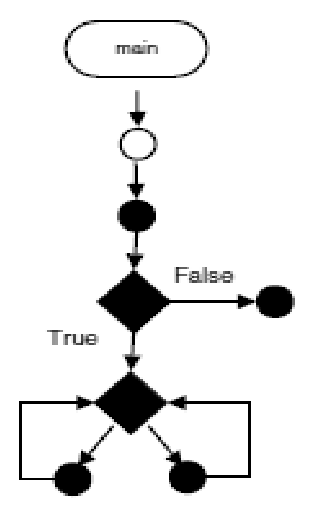
\includegraphics[scale=0.35,clip]{fig/la.eps} 
\caption{\label{fig:la}Example of Look-Ahead (LA) Heuristic} 
\end{figure}

The key idea of the Look-Ahead (LA) heuristic is to perform a reachability analysis in terms of reachable items in the CFG, and decide whether the current
path must be expanded based on the reachability analysis. If no new items can be reached, then exploration along the current path is stopped.

Figure \ref{fig:la} shows an example for illustrating the Look-Ahead (LA) heuristic. Let us assume the depth bound $k \geq 4$ and the objective is to achieve full statement coverage, and every path of the program is feasible. Then the original DFS based produre needs to explore $\approx2^k$ paths to achieve full coverage (because of the two nested loops) while DFS+LA requires at most 3 paths: one path to cover the false branch and two paths to cover two loops.

\subsection{Max-CallDepth (MCD) heuristic}
The major source of path explosion is function calls, and especially nested function calls. It is more embarrassing when only the top-level function is of interest. For example, it may be the case that the procedure explores alternative (long) paths due to backtrack in deep callees while a simple backtrack at top-level would be sufficient. Example of figure \ref{fig:mcd} gives such a behaviour.

\begin{figure}
\centering
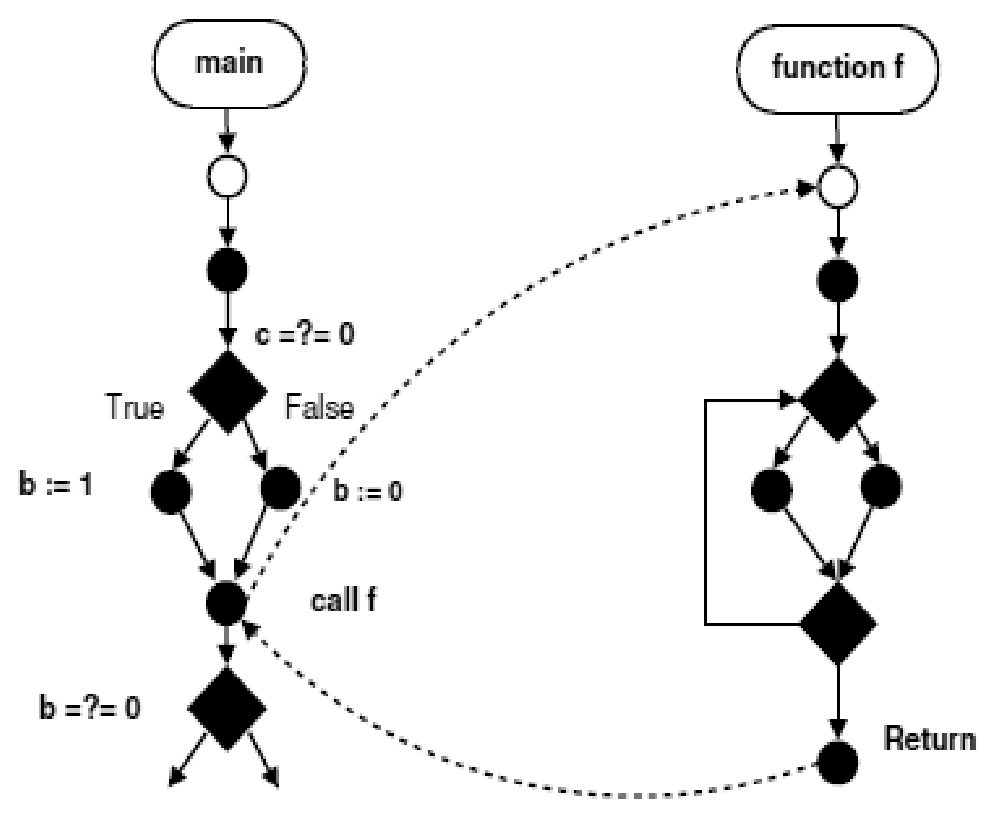
\includegraphics[scale=0.35,clip]{fig/mcd.eps} 
\caption{\label{fig:mcd}Example of Max-CallDepth (MCD) heuristic} 
\end{figure}

The principle of the Max-CallDepth heuristic (MCD) is to prevent backtracking in deep nested calls, hoping such a deep decision is not mandatory to cover the function under test. It is clear that this heuristic makes sense only in unit testing. Moreover, contrary to LA, MCD may discard relevant paths and prevent the full coverage of the function under test. On the other hand, on some programs MCD can discard many paths and still achieve full coverage. These results are summarised in the next property.

\subsection{Solve-First (SF) heuristic}




\section{AI in Fault Detection}
A software fault (also called bug) refers to a static defect in the software. When the software is executed with a certain input, a software fault may result in an incorrect internal state, which is referred to as software error. If the software error is propogated to the output of the software, and results in incorrect behaviors with respect to the requirements or other description of the expected behavior, a software failure occurs~\cite{testbook}. 

As the size of complexity of software has grown quickly in past decades, the difficulty of finding and fixng software faults has increased. Among the different types of faults, concurrency faults are the most notorious, due to their non-deterministic nature. Concurrency faults depend not only on inputs and execution environments, but also on threadinterleaving and other timing-related events that are to be manifested, which creates challenges to expose and detect concurrency faults during in-house testing. With the pervasiveness of multi-core machines and concurrent programs, this problem is becoming more and more severe.

Besides concurrency faults, semantic faults are another form of hard-to-detect faults. Typical semantic faults are caused by missing the reassignment of some variables or incorrectly reuse some variables. Such faults are program-specific and difficult to detect by using only in-housing testing. Finally, memory corruption faults such as buffer overflow and dangling pointer are also important, since they can be exploited by malicious users.

To automatically identify such faults, Shi et al.~\cite{wrongDefinition} proposes an approach to first learn the Definition-Use Invariants and then use the learned knowledge of Definition-Use for detecting faults. They observed that regardless of the difference between these faults' root causes, many of them share a common characteristic: when triggered, they usually are followed by an incorrect data flow, i.e., a read instruction uses the value from an unexpected definition, referred to as an incorrect definition. Such commonality indicates that, if we can detect such incorrect definition-use data flow, it is possible to identify these faults automatically, regardless of their different root causes.

Their approach leverages in-house testing as training runs to extract the definition-use invariants. To tolerate insufficient training, their approach automatically prunes out unlikely invariants and violations, and ranks remaining violations based on confidence. Their approach also considers possible training noises (which
may be incorrectly labeled training runs).

\subsection{Definition-Use Invariants}
\textbf{Local/Remote (LR) Invariants.} In concurrent programs, certain read instructions may use only local definitions or only remote definitions (maybe for the purpose of communication or synchronization). LR invariants can be used to describe these properties. Formally speaking, an LR invariant, $LR(r)$, at a read instruction, $r$, equals to “LOCAL” (respectively “REMOTE”) if $r$ uses only definitions from the local (respectively remote) thread. Such invariants are denoted as LR-Local and LR-Remote, respectively. If $r$ can read from either a local or a remote definition, $r$ has no LR invariant. Figure \ref{fig:invariants}(a) illustrates the basic idea of LR invariant.

\begin{figure}
\centering
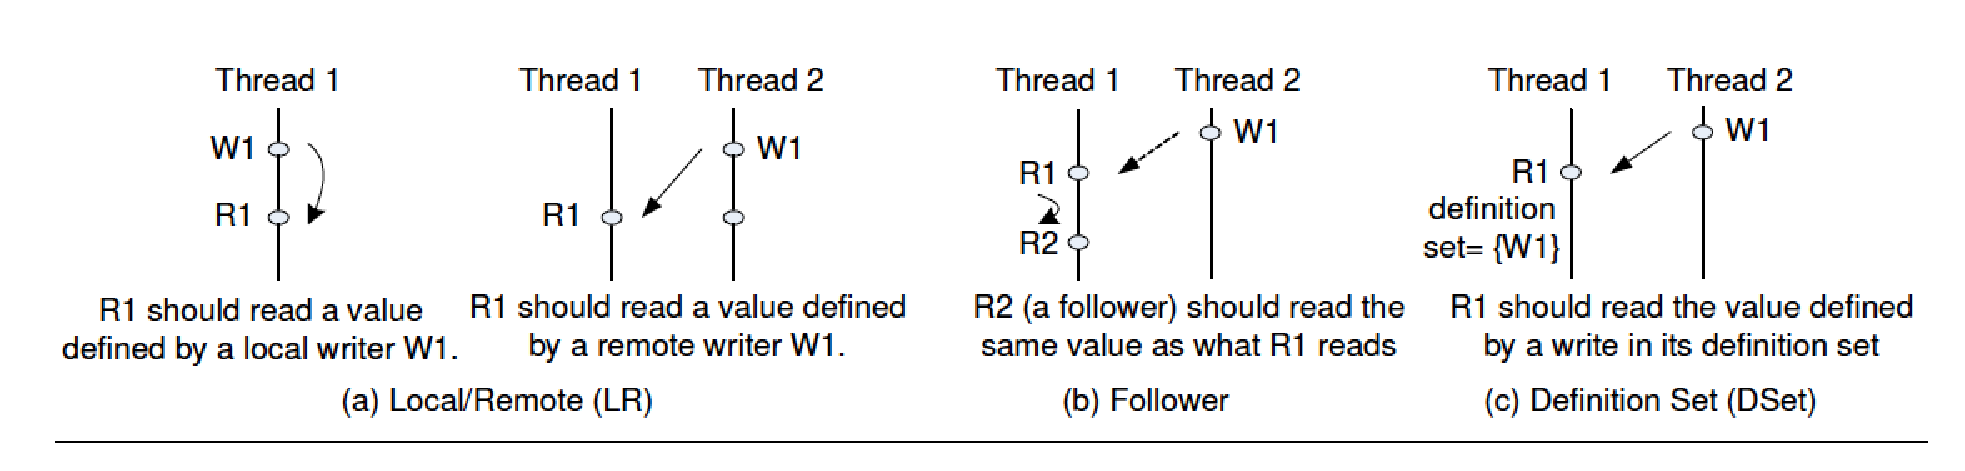
\includegraphics[scale=0.5,clip]{fig/invariants.eps} 
\caption{\label{fig:invariants}Examples of real-world definition-use invariants and their violations.} 
\end{figure}

\textbf{Follower Invariants.} In concurrent programs, developers tend to make assumptions about the atomicity of certain code regions. The LR invariants already captures the case of read-after-write data flow relation in an assumed atomic region, but not the read-after-read case, which can be captured by using a Follower Invariant. Specifically, for two consecutive reads, $r1$ and $r2$, to the same location from the same thread, if $r2$ always uses the same definition as $r1$, $r2$ has a Follower invariant. Follower is different from LR because as long as $r2$ uses the same definition as $r1$, the definition can come from either local or remote. Figure \ref{fig:invariants}(b) demonstrates Follower invariants.

\textbf{Definition Set (DSet) Invariants.} Although concurrent programs have special inter-thread data flows, definition-use is not specific to only concurrent programs. Definition Set (DSet) invariant is suitable for identify faults in both sequential and concurrent programs. A DSet invariant at a read instruction is defined as the set of all write instructions whose definitions this read instruction may use. Figure \ref{fig:invariants}(c) shows a DSet invariant at $R1$. Every read instruction has such a DSet. When an instruction violates a DSet invariant by consuming a value defined by an instruction outside its DSet, this instruction may indicate a likely fault.


\subsection{Invariant Extraction}
To identify faults using definition-use invariants, their approach consists of two phases: (1) an extraction phase for inferring definition-use invariants; and (2) a detection phase for detecting invariant violations and reporting potential faults after pruning and ranking. Figure \ref{fig:overview} shows the overview of their approach.

\begin{figure}[b]
\centering
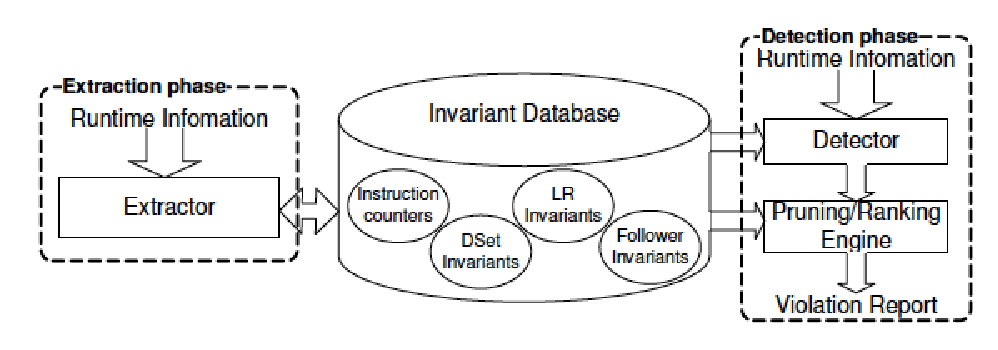
\includegraphics[scale=0.6,clip]{fig/overview.eps} 
\caption{\label{fig:overview}Overview of fault detection using definition-use invariants.} 
\end{figure}

\textbf{DSet invariant extraction}. Their approach obtains DSet by collecting all definitions that are used
by $I_U$ (read instruction) during training runs. For each memory location, their approach stores its most recent $I_D$ (write instruction) in a global hash-table, called Definition-Table. At a read instruction $i_u$, their approach retrieves its definition id from the Definition-Table and uses id's corresponding static instruction ID to update $I_U$'s DSet:

$$ DSet(I_U) \leftarrow DSet(I_U) \bigcup \{I_D\}$$

After the training phase, information for every instructions' DSet is stored into the invariant database along with some statistical information such as the number of times $I_U$ and $I_D$ are executed, and so on. Such statistical information is used for the purpose of pruning and ranking in later phases.

\textbf{LR invariant extraction.} In order to infer LR invariants, their approach first obtains the knowledge of which thread provides the definition for a read instruction by using the Definition-Table. In particular, when $i_u$ is executed, their approach identifies its definition id from the Definition-Table. Their approach then compares the thread identifiers, $T(iu)$ and $T(id)$, to determine whether they are from the same thread or not. Finally, their approach compares the answer with the LR($I_U$) associated with $I_U$. If they are different, LR($I_U$) is set to NO INV to indicate that there is no LR invariant at $I_U$ and this read instruction is no longer monitored for LR invariant extraction. LR($I_U$) is initialized based on the
definition source (either REMOTE or LOCAL) on the first time $I_U$ is executed. This process can be formalized as follows:

\[
LR(I_U) \leftarrow 
\begin{cases}
LOCAL, \text{if } LR(I_U) = LOCAL \wedge T(i_d) = T(i_u)\\
REMOTE, \text{if } LR(I_U) = REMOTE \wedge T(i_d) <> T(i_u)\\
NO\_INV, \text{Otherwise } 
\end{cases}
\]

\textbf{Follower invariant extraction.} To infer Follower invariants, their approach stores its recent access history to determine whether an instruction and its predecessor use the same definition. Their approach maintains a bitvector for every memory location $m$, called has $read(m)$. A bit in the vector has $read(m,t)$ indicates whether the current definition to memory location $m$ has already been used by thread $t$. By checking this bit-vector before every read instruction $i_u$, their approach can easily determine whether $i_u$
and its predecessor use the same definition.

In particular, bit-vector has $read(m)$ is initialized as zero. Every write to $m$ sets all bits of $has\_read(m)$ to zero. After any read from $m$ in thread $t$, $has\_read(m, t)$ is set to one. Before executing a read instruction $i_u$, their approach checks if the corresponding bit (i.e., $has\_read(m,t)$) is one. If it is, it means that there is no new definition since thread $T(i_u)$'s last use to $m$. In other words, $i_u$ shares
the same definition with its predecessor.

To maintain and update the Follower invariant information for $I_U$, their approach associates Follower($I_U$ ) with it. This flag is set to $TRUE$ if $I_U$'s dynamic instances always share definition with their predecessors. Whenever a dynamic instance of $I_U$ uses a different definition from its predecessor, the flag is set to $FALSE$ and $I_U$ is no longer monitored for Follower invariant extraction.

$$ Follower(I_U) \leftarrow Follower(I_U) \wedge has\_read(m,T(i_u))$$


\subsection{Fault Detection}
To detect DSet invariant violation, their approach maintains a Definition-Table at runtime so that it knows which instruction provides a definition for each use. If the definition for a use is not in this use's DSet, a violation is issued. Formally speaking, the violation condition is:
$$I_D \notin DSet(I_U)$$

Detecting violations against LR invariants is also straightforward. At a monitored read, their approach checks whether this read has an LR invariant or not. If it does, their approach examines whether the monitored read and its definition come from the same thread and matches the monitored condition with the type of LR invariant (LOCAL and REMOTE) extracted at this read instruction. 
$$\{LR(I_U) = LOCAL \wedge T(i_d) <> T(i_u)\} \vee \{LR(I_U) = REMOTE \wedge T(i_d) = T(i_u)\}$$

To detect violations to Follower invariants, their appraoch checks whether an instruction with a Follower invariant shares the same definition with its predecessor (by leveraging the has $read(m)$ vector similar to that used in extraction). If not, a violation will be reported.
$$Follower(I_U) \wedge \overline{has\_read(m,T(i_u))}$$

\subsection{Pruning and Ranking}
\textbf{Pruning.} Their approach automatically prunes the following cases: (1) \textit{Barely exercised uses}: For read instructions that are never covered during training, their approach do not report any violations since their approach do not extract any invariants associated with them; (2) \textit{Barely exercised definitions}: For definitions that are never exercised during training runs, their approach also prunes them; (3) \textit{Popular uses}: Some uses, such as those in a small function called from multiple call-sites, are very popular and have a large definition set. In this case, their approach also prunes it as it might be perfectly acceptable to have yet another definition for this use during detection runs.

\textbf{Ranking.} After pruning the above cases, their ranks every unpruned violations based on its confidence. Their approach relies on the following conditions to increase the confidence of a fault: (1) many dynamic instances of the definition ($\#I_D$) and the use ($\#I_U$) during training; (2) no significant difference between the number of instances of the definition and instances of the use ($|\#ID - \#IU|$) during training; (3) small definition set ($|DSet(I_U)|$); (4) few instances of this violation pair ($\#violation_{DSet}(I_D, I_U)$) during detection.

For violations to DSet invariants, their approach computes the confidence using the following formula:
$$conf_{DSet} = \frac{\#I_D \times \#I_U}{(|\#ID - \#IU| \times |DSet(I_U)| \times \#violation_{DSet}(I_D, I_U))}$$

For LR and Follower violations, the confidence is computed based only on the number of dynamic instances of a
use during training and the number of violations occurring during detection, as follows:
$$conf_{LR}=\#I_U / \#violation_{LR}(I_U)$$
$$conf_{F}=\#I_U / \#violation_{F}(I_U)$$

\subsection{Conclusion}
Shi et al.~\cite{wrongDefinition} proposed definition-use invariants which can be used to detect a wide range of software faults, including both concurrency bugs (atomicity and order violations) and sequential bugs (memory corruptions and certain semantic faults). Their experimental results with 16 real-world applications and 20 real-world faults of different types have shown that their approach was effective in detecting 19 of them, including 2 new faults that were never reported before, while introducing only 0-3 false positives. Their training sensitivity experiments showed that their approach can reasonably tolerate insufficient training, especially with confidence-based pruning.

% Recent research works~\cite{wrongDefinition,online} that use AI techniques have advanced the research in reducing the human efforts on fault detection: Shi et al.~\cite{wrongDefinition} proposes an approach to first learn the Definition-Use Invariants and then use the learned knowledge of Definition-Use for detecting concurrency and sequential bugs; Baah et al~\cite{online} and proposes a new machine-learning technique that performs fault detection for deployed software. I plan to study in details how these research works adopt the concepts and techniques of AI to assist the task of fault detection.

\section{AI in Software Repair}

Symbolic execution~\cite{symbolic} is used to reason path-flow behavior of a program by tracing path constraint information collected during symbolic execution. This technique is useful in automated software testing such as increasing path coverage.

There exist two issues with regards to limited scalability of symbolic execution. The first issue is that this technique can be applied on only small program with at most thousands of lines of code. Note that symbolic execution collects states and constraints to keep track of path information in a program. During symbolic execution, the size of such states and constraints is exponential to the number of conditions (e.g., as if-else statements in program) in a program. This problem is called as path explosion. Due to such an exponential growth, the technique is not yet applied to large programs (e.g., program with more than millions lines of code).

The second issue is related to symbolic execution interacting with environments such as library or third-party program. Many programs are often interacting with environments such as external libraries to control network devices. For example, if a program under test uses external libraries, the program may require symbolic execution on external libraries as well. Such symbolic execution of environments could result in path explosion.

Ideally, testers often try to achieve covering all or specific paths of a system. However, in practice, covering such paths is not trivial due to limited scalability caused by path explosion. To address the issue, Chipounov et al.~\cite{selective} propose selective symbolic execution technique. The main idea of this technique, called selective symbolic execution (S$^2$E), combines both symbolic execution and concrete execution. More specifically, users specify portions (in a system) of interest. For example, portions of interest could be program related to CPU or memory usage to detect deadlock or memory leakage. S$^2$E explores such portions (of interest) symbolically (i.e., in-scope executions) and the remaining portions (of non-interest) concretely (i.e., out-scope executions). Therefore, execution of a program under test is back and forth between the symbolic and concrete executions based on which portions are executed.

S$^2$E can be practical since the authors observe that developers often focus on only small portion of code in a system (e.g., kernel module or newly added feature) instead of testing a whole system. S$^2$E can be useful for many important software development tasks as follows.

\begin{figure}
\centering
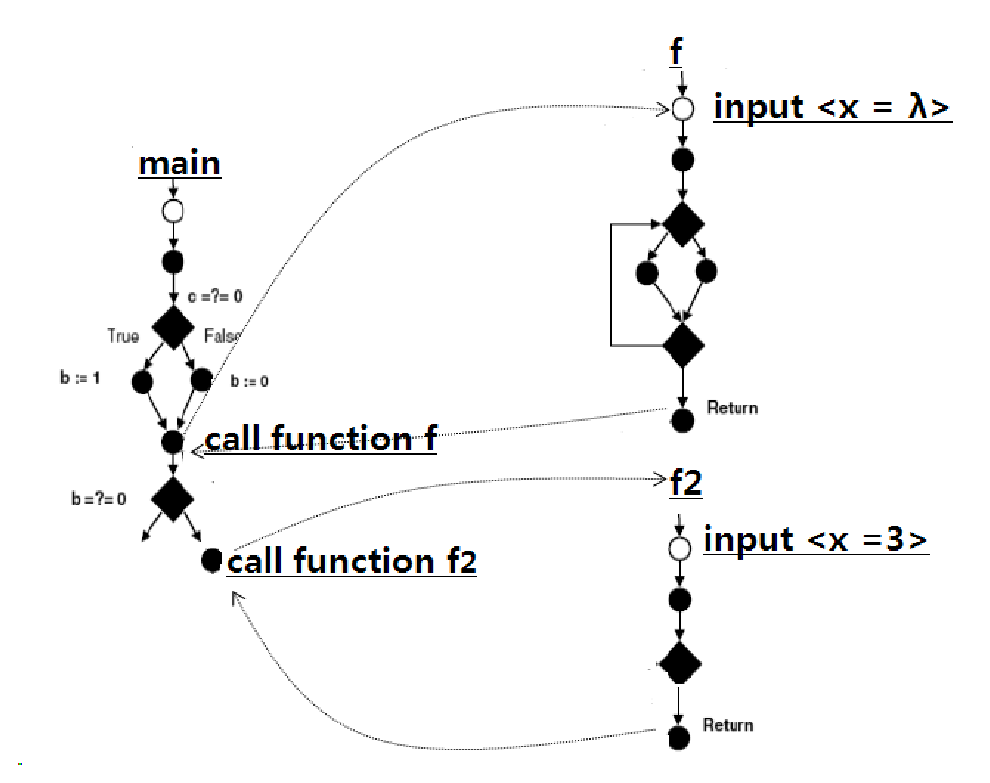
\includegraphics[scale=0.6,clip]{fig/selective.eps} 
\caption{\label{fig:s2e}Example of selective symbolic execution} 
\end{figure}


Selective symbolic execution (S$^2$E) has two dimensions in a system; code and data. Users can specify portions of code of interest by indicating file name or range of program counters. Given code information, S$^2$E executes the portion of code symbolically. All variables in the portion in conditional branches are involved in symbolic execution. Therefore, all paths could be explored symbolically. Users can specify portions of data of interest by indicating a data structure's name or address range of data segment. Then, S$^2$E executes all portion of code related to the data of interest symbolically.
Figure~\ref{fig:s2e} shows an example of S$^2$E execution. In the example, the main function calls functions $f$ and $f_2$. Consider that users specify $f$ is portion (of interest) to be executed symbolically. To achieve the goal, when the main function calls the $f$ that has an input parameter $X$, $X$ is assigned to a symbolic value, $\lambda$ and $f$ is symbolically executed. However, when the main function calls the $f_2$ of non-interest, S$^2$E assigns $X$ as ``3'' to execute $f_2$ concretely.




\bibliographystyle{plain}
\bibliography{references}
\end{document}